\begin{frame}{4.1 Recommandation, collaborative filtering}
  \begin{itemize}
  \item Algorithme classique de \textcolor{orangeAgaetis}{recommandation de produits}
  \item Utilise les \textcolor{orangeAgaetis}{notes} donné à chaque produit par les utilisateurs
  \item \textcolor{orangeAgaetis}{Vainqueur du challenge Netflix} (et toujours utilisé)
  \end{itemize}
  \vfill
  \begin{minipage}{0.35\textwidth}
    \begin{figure}
      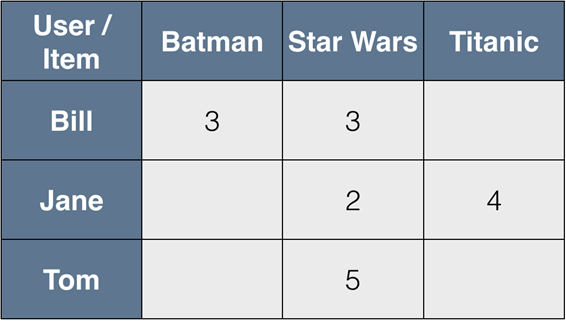
\includegraphics[width=0.9\textwidth]{figs/collabFilteringEx}\put(-88,26.5){\textcolor{black}{1}}\put(-94,8){\textcolor{red}{2.38}}
    \end{figure}
  \end{minipage}
  \hfill
  \begin{minipage}{0.6\textwidth}
    \begin{itemize}
    \item \textcolor{orangeAgaetis}{Degré de similarité} entre utilisateurs (ou produits)
      \begin{itemize}
      \item Similarité \textcolor{orangeAgaetis}{Cosinus} ou \textcolor{orangeAgaetis}{Pearson}
      \end{itemize}
    \item Estimation de l'intérêt d'un utilisateur pour un produit en se basant sur les utilisateurs similaires:
    \end{itemize}
    \begin{equation*}
      cosSim(Bill, Tom) = 0.71 ~/~ cosSim(Jane, Tom) = 0.32
    \end{equation*}    
  \end{minipage}
  \vfill
  \begin{itemize}
  \item Filtrage \textcolor{orangeAgaetis}{actif}: l'utilisateur donne des notes/son avis
  \item Filtrage \textcolor{orangeAgaetis}{passif}: Il faut déduire les goûts de l'utilisateur via son comportement
  \item \textcolor{orangeAgaetis}{Limites:} temps de calcul, nouveaux arrivants, comportements singuliers
  \end{itemize}
\end{frame}

\begin{frame}{4.1 Recommandation, collaborative filtering, formules}
  \begin{itemize}
  \item \textcolor{orangeAgaetis}{Similarité Pearson:} $sim(x, y) = \frac{\displaystyle\sum_{i \in I_{xy}}(r_{x,i} - \bar{r_{x}})(r_{y,i} - \bar{r_{y}})}{\sqrt{\displaystyle\sum_{i \in I_{xy}}(r_{x,i} - \bar{r_{x}})^{2}}\sqrt{\displaystyle\sum_{i \in I_{xy}}(r_{y,i} - \bar{r_{y}})^{2}}}$
  \item \textcolor{orangeAgaetis}{Similarité Cosinus:} $simCos(x,y) = cos(\vec{x}, \vec{y}) = \frac{\vec{x} . \vec{y}}{\|\vec{x}\| \times \|\vec{y}\|} = \frac{\displaystyle\sum_{i \in I_{xy}} r_{x,i}r_{y,i}}{\sqrt{\displaystyle\sum_{i \in I_{x}}r_{x,i}^{2}}\sqrt{\displaystyle\sum_{i \in I_{y}}r_{y,i}^{2}}}$
  \item \textcolor{orangeAgaetis}{Estimation:} $r_{u,i} = \frac{\displaystyle\sum_{u' \in U} sim(u, u')r_{u',i}}{\displaystyle\sum_{u' \in U} |sim(u,u')|}$
  \end{itemize}
\end{frame}

\begin{frame}{4.2 Optimisation, algorithme génétique}
  \begin{itemize}
  \item Algorithme d'optimisation par sélection/mutation successives
  \item Réponds aux problèmes à forte combinatoire sans solution unique
  \item Détermine le jeu des solutions optimales (front de Pareto)
  \end{itemize}
  \begin{minipage}{.65\textwidth}
    \begin{itemize}
    \item \textcolor{orangeAgaetis}{\textbf{population de solutions}}:
      \begin{itemize}
      \item \textcolor{orangeAgaetis}{Initialisation $\rightarrow$ Selection $\rightarrow$ Reproduction $\rightarrow$ Mutation}
      \end{itemize}
    \end{itemize}
    \vfill
    \hspace{0.25\textwidth}
    \begin{minipage}{0.5\textwidth}
      \begin{figure}
        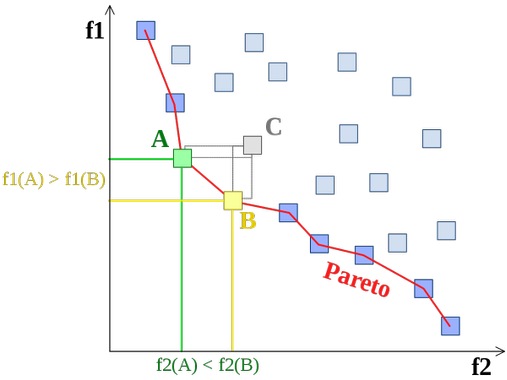
\includegraphics[width=\textwidth]{figs/Front_pareto.png}
      \end{figure}
    \end{minipage}
  \end{minipage}
  \begin{minipage}{.3\textwidth}
    \begin{figure}
      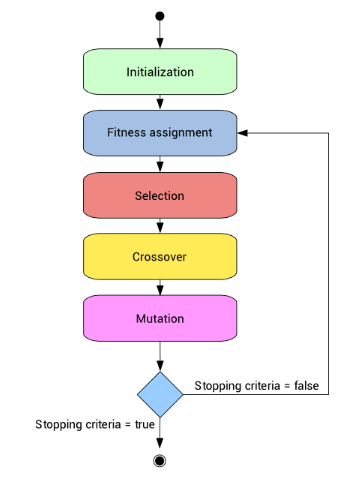
\includegraphics[width=0.9\textwidth]{figs/genAlg_desc.png}
    \end{figure}
  \end{minipage}
\end{frame}

\begin{frame}{4.2 Optimisation, algorithme génétique}
  \begin{itemize}
  \item Applications:
    \begin{itemize}
      \normalsize
    \item Voyageur de commerce
    \item Sélection de features
    \item Hyper-paramètrage algorithme ML
    \item $\dots$
    \end{itemize}
  \end{itemize}
  \vfill
  \begin{minipage}{0.35\textwidth}
    \vspace{0.5cm}
    \animategraphics[autoplay,loop,height=0.38\textheight]{5}{figs/gif/ag/3bd2f86e4098463caf88e538c6a9746e-}{0}{48} %% Insert gif as png list    
  \end{minipage}
  \begin{minipage}{0.41\textwidth}
    \vspace{0.5cm}
    \begin{figure}
      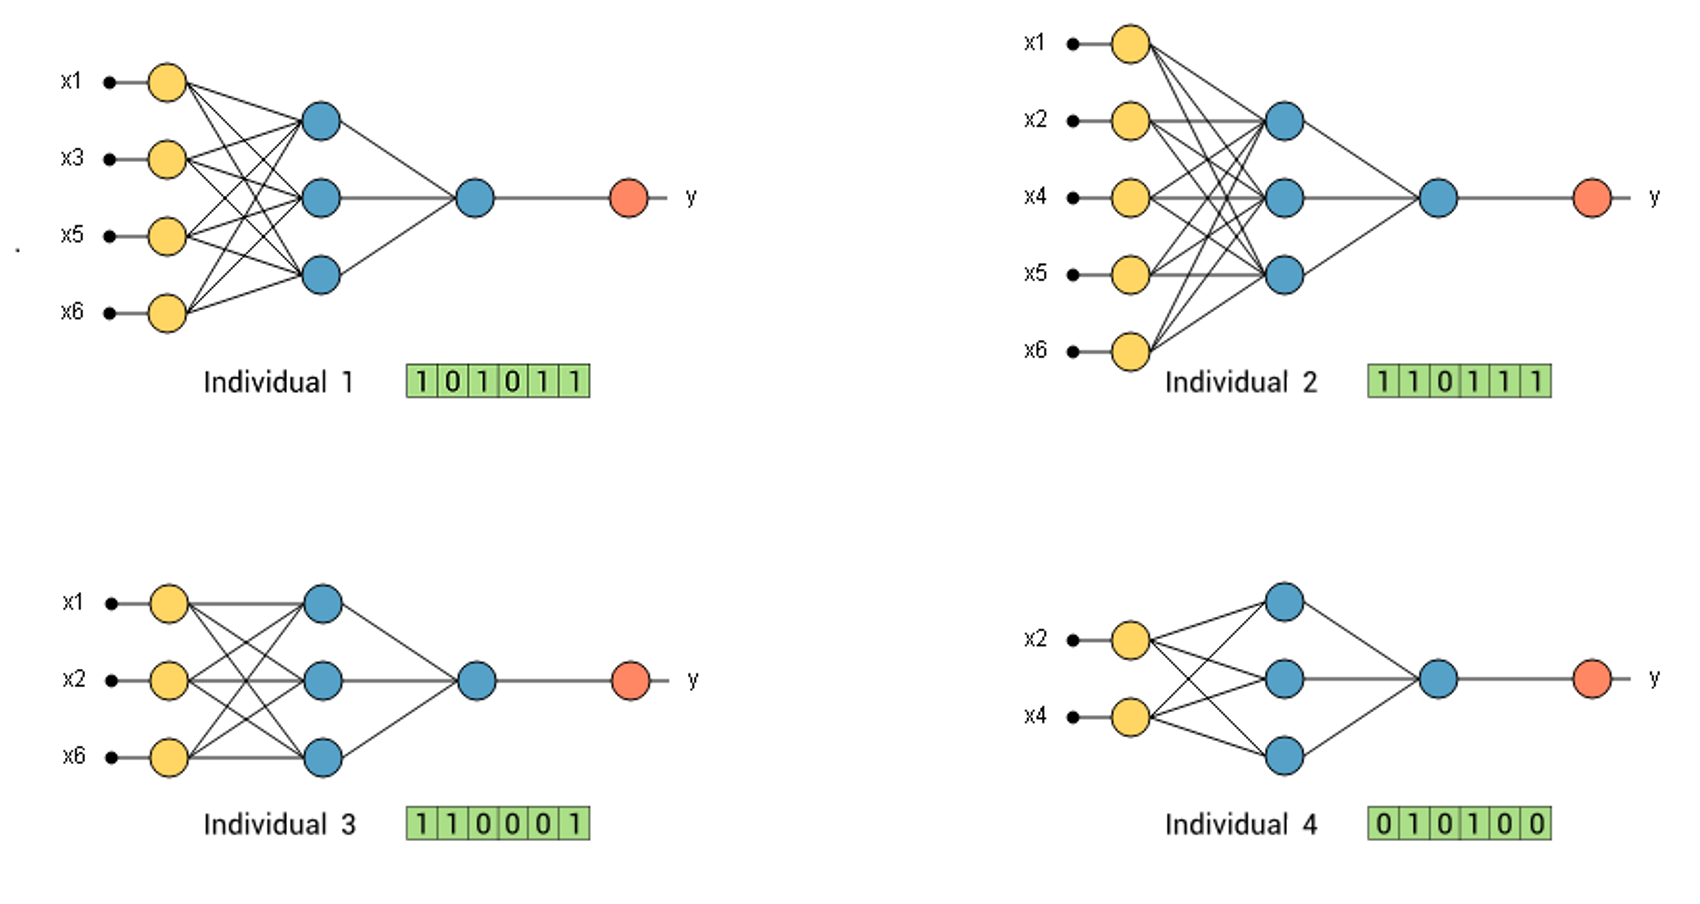
\includegraphics[height=0.38\textheight]{figs/individuals_network.png}
    \end{figure}
  \end{minipage}
  \begin{minipage}{0.22\textwidth}
    \vspace{0.5cm}
    \begin{figure}
      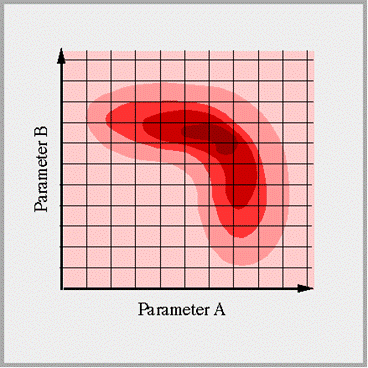
\includegraphics[height=0.38\textheight]{figs/gridsearch.png}
    \end{figure}
  \end{minipage}
\end{frame}
